\documentclass{article}
\usepackage[utf8]{inputenc}
\usepackage[english]{babel}
\usepackage{geometry}
\usepackage{amsmath}
\usepackage{graphicx}
\graphicspath{ {./images/} }
\usepackage{hyperref}
\usepackage{array}
\usepackage{adjustbox}
\usepackage{pdflscape}
\usepackage{hhline}
\usepackage{color}
\usepackage{tikz}
\usepackage{forest}
\usepackage{algorithmic}
%\usepackage[ruled,vlined]{algorithm2e}
\usepackage{algorithm}
\usepackage{float}
\usepackage{diagbox}
\usepackage{setspace}
\usepackage{wrapfig}
\usepackage{multirow}
\usepackage{listings}
\usepackage{indentfirst}
\usepackage{changepage}



\lstset
{
    breaklines=true,
    breakatwhitespace=true,
    frame=lines,
    columns=fullflexible,
    basicstyle=\ttfamily,
}

\onehalfspacing

\geometry{top=100px, bottom=100px, left=75px, right=75px}

\begin{document}
\begin{titlepage}
    \begin{center}
        \vspace*{1cm}


        \Huge
        \textbf{Advanced Databases}
        \vspace{0.25cm}

        \LARGE
        \textbf{INFO-H-415}

        \vspace{0.25cm}
        \LARGE
        \text{Final Project}

        \vspace{0.25cm}
        \textit{31 January 2020}

        \vspace{3cm}
           \Large
        \textbf{BAKKALI Yahya : 000445166 \\}
        \textbf{HAUWAERT Maxime : 000461714 \\}

        \vspace{2cm}

        \textsc{Université Libre de Bruxelles (ULB)}


    \end{center}
\end{titlepage}

\tableofcontents
\newpage


\section{Introduction}
The goal of this project is to perform multiple queries on a graph based version of DBLP using Neo4j. DBLP is a online bibliographical database for computer science. Neo4j is a database management system based on graphs. The process of loading the \texttt{XML} DBLP database into Neo4j will be seen as well as twenty different interesting queries in the domain of academic publications. After that the performances of the different queries on four different databases of different sizes will be seen.

\section{Loading}
DBLP is a database that is distributed in a \texttt{XML} format file, so a solution to load this type of format into Neo4j was needed. The web offers many solutions but none of them was appropriate for this project as they did not fully use the power of graph databases.

To tackle this problem it has been decided to create a python3 program that takes the path of the \texttt{XML} file and create all the nodes and relations needed. It was possible to load directly the \texttt{XML} file via a Cypher command with the help of the \texttt{APOC} plugin, but it could only load little databases due to some memory problems related to the java heap space. The python3 program takes a long time to load the databases, more than two hours and a half for an excerpt of the DBLP database that contains 50000 publications, but it is the price to pay to fully take advantage of the graph database.

The python script parse the \texttt{XML} file and for each publication it generates a query that creates all the nodes and relations needed and when there are no information left it sends the query to Neo4j that executes it and then goes to the next publication. By doing this it solves the memory problems.

Some arbitrary decision have been made. When a publication cites another publication that is not in the DBLP database, the key is represented by three dots, it has been decided to ignore them.

In the two next subsections will be seen all the different relevant types of nodes and relations that have been created to manipulate in an efficient way the data of DBLP.

\subsection{Nodes}
Here is a list of all the types of nodes created as well as all the attributes they can have.

\subsubsection{Publication}
This label is used to regroup all the publications under a same label. Generally the nodes with this label have another label that specifies their types. It must have a key attribute and it can have these attributes : title, booktitle, pages, address, volume, number, month, url, ee, cdrom, note, crossref, isbn, series, chapter, publnr, mdate, publtype, reviewid, rating, cdate.

Here is all the type of publications : Article, Inproceedings, Proceedings, Book, Incollection, PHDThesis, MasterThesis, WWW.

\subsubsection{Person}
This label represent a person and it must have a name attribute. The name represents the full name of the person. Two people cannot have the same name.

\subsubsection{Journal}
This label represent a journal and it must have a name attribute. Two journals cannot have the same name.

\subsubsection{Publisher}
This label represent a publisher and it must have a name attribute. Two publishers cannot have the same name.

\subsubsection{School}
This label represent a school and it must have a name attribute. Two schools cannot have the same name.

\subsubsection{Series}
This label represent the series of books and it must have a name attribute. Two series of books cannot have the same name.

\subsubsection{Year}
This label represent a year and it must have a year attribute. Two years cannot be the same.

\subsection{Relations}

\subsubsection{author}
This relation goes from a publication to a person. It means that the person is an author of the publication.

\begin{center}
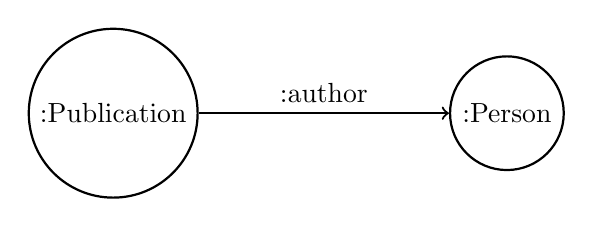
\begin{tikzpicture}[node distance={50mm}, thick, main/.style = {draw, circle}] 
\node[main] (1) {:Publication};
\node[main] (2) [right of=1] {:Person};
\draw[->] (1) -- node[midway,above] {:author} (2);
\end{tikzpicture} 
\end{center}

\subsubsection{editor}
This relation goes from a publication to a person. It means that the person is an editor of the publication.

\begin{center}
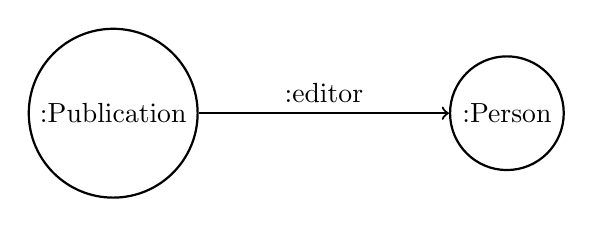
\begin{tikzpicture}[node distance={50mm}, thick, main/.style = {draw, circle}] 
\node[main] (1) {:Publication};
\node[main] (2) [right of=1] {:Person};
\draw[->] (1) -- node[midway,above] {:editor} (2);
\end{tikzpicture} 
\end{center}

\subsubsection{cite}
This relation goes from a publication to another publication. It means that the first publication cites the second publication.

\begin{center}
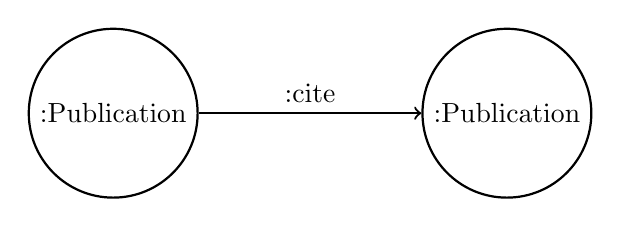
\begin{tikzpicture}[node distance={50mm}, thick, main/.style = {draw, circle}] 
\node[main] (1) {:Publication};
\node[main] (2) [right of=1] {:Publication};
\draw[->] (1) -- node[midway,above] {:cite} (2);
\end{tikzpicture} 
\end{center}

\subsubsection{journal}
This relation goes from a publication to a journal. It means that the publication was published in the journal.

\begin{center}
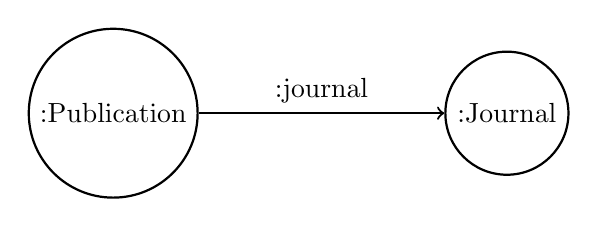
\begin{tikzpicture}[node distance={50mm}, thick, main/.style = {draw, circle}] 
\node[main] (1) {:Publication};
\node[main] (2) [right of=1] {:Journal};
\draw[->] (1) -- node[midway,above] {:journal} (2);
\end{tikzpicture} 
\end{center}

\subsubsection{publisher}
This relation goes from a publication to a publisher. It means that the publication was published by the publisher.

\begin{center}
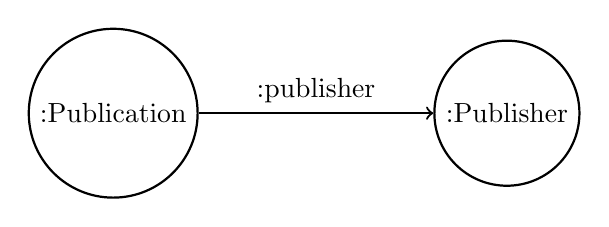
\begin{tikzpicture}[node distance={50mm}, thick, main/.style = {draw, circle}] 
\node[main] (1) {:Publication};
\node[main] (2) [right of=1] {:Publisher};
\draw[->] (1) -- node[midway,above] {:publisher} (2);
\end{tikzpicture} 
\end{center}

\subsubsection{school}
This relation goes from a publication to a school. It means that the publication was written in the school.

\begin{center}
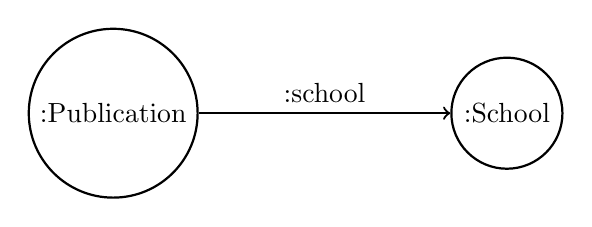
\begin{tikzpicture}[node distance={50mm}, thick, main/.style = {draw, circle}] 
\node[main] (1) {:Publication};
\node[main] (2) [right of=1] {:School};
\draw[->] (1) -- node[midway,above] {:school} (2);
\end{tikzpicture} 
\end{center}

\subsubsection{series}
This relation goes from a publication to a series. It means that the publication belongs to the series.

\begin{center}
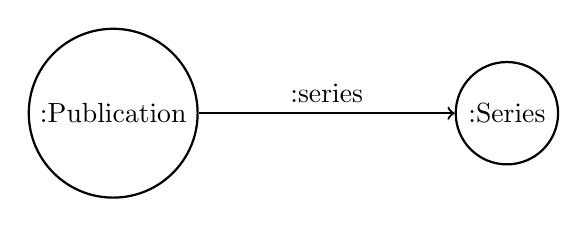
\begin{tikzpicture}[node distance={50mm}, thick, main/.style = {draw, circle}] 
\node[main] (1) {:Publication};
\node[main] (2) [right of=1] {:Series};
\draw[->] (1) -- node[midway,above] {:series} (2);
\end{tikzpicture} 
\end{center}

\subsubsection{crossref}
This relation goes from a inproceedings to a proceedings. It means that the inproceedings is an article in the proceedings.

\begin{center}
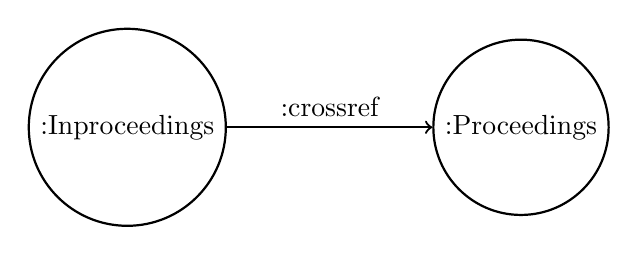
\begin{tikzpicture}[node distance={50mm}, thick, main/.style = {draw, circle}] 
\node[main] (1) {:Inproceedings};
\node[main] (2) [right of=1] {:Proceedings};
\draw[->] (1) -- node[midway,above] {:crossref} (2);
\end{tikzpicture} 
\end{center}

\subsubsection{year}
This relation goes from a publication to a year. It means that the publication has been published in the year.

\begin{center}
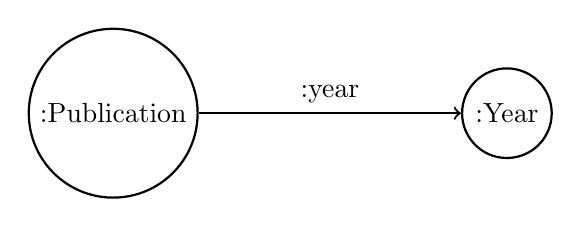
\begin{tikzpicture}[node distance={50mm}, thick, main/.style = {draw, circle}] 
\node[main] (1) {:Publication};
\node[main] (2) [right of=1] {:Year};
\draw[->] (1) -- node[midway,above] {:year} (2);
\end{tikzpicture} 
\end{center}

\section{Queries}
In this project twenty queries aimed at describing various aspects of the dynamics of the domain of academic publications have been implemented in Cypher.


\subsection{Give the number of publications for each type}
This query returns the different types of publications followed by the number of items that composed them.

\begin{lstlisting}
    OPTIONAL MATCH (p:Article) RETURN "Article" as Type, COUNT(p) as Number
    UNION ALL
    OPTIONAL MATCH (p:Inproceedings) RETURN "Inproceedings" as Type, COUNT(p) as Number
    UNION ALL
    OPTIONAL MATCH (p:Proceedings) RETURN "Proceedings" as Type, COUNT(p) as Number
    UNION ALL
    OPTIONAL MATCH (p:Book) RETURN "Book" as Type, COUNT(p) as Number
    UNION ALL
    OPTIONAL MATCH (p:Incollection) RETURN "Incollection" as Type, COUNT(p) as Number
    UNION ALL
    OPTIONAL MATCH (p:PHDThesis) RETURN "PHDThesis" as Type, COUNT(p) as Number
    UNION ALL
    OPTIONAL MATCH (p:MasterThesis) RETURN "MasterThesis" as Type, COUNT(p) as Number
    UNION ALL
    OPTIONAL MATCH (p:WWW) RETURN "WWW" as Type, COUNT(p) as Number
\end{lstlisting}

In order to execute this query it is first needed for each type to match all the publications of the current type and to simply count them, then all the sub-results are regrouped with an \texttt{UNION ALL}. The optional clauses with the matches are necessary as there can be a type of publications that is not in the database but it still will display the type followed by a zero, if the optional was not present the type will simply not appear.


\subsection{Give the name of authors}
This query returns the names of the people who were an author for at least one publication.

\begin{lstlisting}
    MATCH (p:Person)<-[:author]-()
    RETURN DISTINCT p.name as Name
\end{lstlisting}

In order to execute this query it is first needed to match all the persons who were an author and then eliminate the duplicates. The \texttt{DISTINCT} is needed because there may be multiple times the same name as an author can write multiple publications. 


\subsection{Give the names of authors who are also editors}
This query return the names of the persons who were an author for at least one publication and editor for at least one publication.

\begin{lstlisting}
    MATCH ()-[:editor]->(p:Person)<-[:author]-()
    RETURN DISTINCT p.name
\end{lstlisting}

In order to execute this query it is first needed to match all the persons who were an author and an editor and then eliminate the duplicates. The \texttt{DISTINCT} is needed because there may be multiple times the same name as a person can be an author and an editor multiple times. 

\subsection{Give the authors ordered by the number of publications, in descending order}
This query returns for each person their names followed by the number of publications they have done, in descending order.

\begin{lstlisting}
    MATCH (p:Person)
    OPTIONAL MATCH (p)<--(a:Publication)
    RETURN p.name as Person, COUNT(a) as Publications
    ORDER BY Publications DESC
\end{lstlisting}

In order to execute this query it is first needed to match all the people, then to match the publications that have a relation with the current person and to count them, finally to order the results in descending order.

\subsection{Give the most active publishers by year} \label{3.5}
This query returns for each year the year followed by the name of the publisher that have published the maximum number of publications.

\begin{lstlisting}
    MATCH (y:Year)-[:year]-(a:Publication)-[:publisher]-(p:Publisher)
    WITH y, p, COUNT(a) as ca 
    ORDER BY ca DESC
    RETURN y.year as Year, collect(p)[0].name as Publisher 
    ORDER BY Year
\end{lstlisting}

In order to execute this query it is first needed to match a publication that have a relation with a publisher and a year, then to count the number of publications by year, finally take the the publisher that has the maximum number of publications. The collect(p)[0] statement return the publisher that has the maximum number of publications for the year with the help of the ORDER BY DESC statement above. 

\subsection{Give the author(s) having the highest number of publications}
This query returns the name of the author(s) who have the highest number of publications.

\begin{lstlisting}
    MATCH (p:Person)<--(a:Publication)
    WITH p, COUNT(a) as c
    WITH max(c) as m
    MATCH (p:Person)<--(a:Publication)
    WITH p, COUNT(a) as c, m
    WHERE c = m
    RETURN p.name as Name
\end{lstlisting}

In order to execute this query it is first needed to calculate the maximum number of publications for an author, then to mach all the authors who have their number of publications equal to the maximum. Another method is, after the count, to order the results in descending order then to do a limit 1, but this method does not take into account that there may be ties, two or more authors that have the highest number of publications. The first method seen is more costly than the second one, but it offers more correct and precise results.


\subsection{Give for each author the total number of publications and the number of publications by type}
This query returns for each author their names followed by the number of publications for each type of publications they have done and the total.

\begin{lstlisting}
    MATCH (p:Person)

    OPTIONAL MATCH (p)<--(a:Article)
    WITH p, COUNT(a) as ca
    
    OPTIONAL MATCH (p)<--(b:Inproceedings)
    WITH p, ca, COUNT(b) as cb
    
    OPTIONAL MATCH (p)<--(c:Proceedings)
    WITH p, ca, cb, COUNT(c) as cc
    
    OPTIONAL MATCH (p)<--(d:Book)
    WITH p, ca, cb, cc, COUNT(d) as cd
    
    OPTIONAL MATCH (p)<--(e:Incollection)
    WITH p, ca, cb, cc, cd, COUNT(e) as ce
    
    OPTIONAL MATCH (p)<--(f:PHDThesis)
    WITH p, ca, cb, cc, cd, ce, COUNT(f) as cf
    
    OPTIONAL MATCH (p)<--(g:MastersThesis)
    WITH p, ca, cb, cc, cd, ce, cf, COUNT(g) as cg
    
    OPTIONAL MATCH (p)<--(h:WWW)
    WITH p, ca, cb, cc, cd, ce, cf, cg, COUNT(h) as ch
    
    RETURN p.name as Person, ca as Article, cb as Inproceedings,
    cc as Proceedings, cd as Book, ce as Incollection, cf as PHDThesis,
    cg as MastersThesis, ch as WWW, ca + cb + cc + cd + ce + cf + cg + ch as Total
\end{lstlisting}

In order to execute this query it is first needed to match a person, then for each type match the publications of this type that have a relation with the current person and to count them, finally sum the number of all the different types of publications. The match for each type are optional because when there are no relations between this type of publications and the person it means that the person has never done this type of publications.

\subsection{Give the list of proceedings that have at least one editor that is also author of at least one article in the proceedings}
This query returns the title of the proceedings that have at least one editor that is also an author of one of their articles.

\begin{lstlisting}
    MATCH (p:Proceedings)-[:editor]-(a:Person), (a)-[:author]-(:Inproceedings)-[:crossref]-(p)
    RETURN DISTINCT p.title as Proceedings
\end{lstlisting}

In order to execute this query it is first needed to match a person that has a relation of the type \texttt{editor} with a proceedings and the same person has a relation of type \texttt{author} with an inproceedings that has a relation of type \texttt{crossref} with the same proceedings, finally eliminate the duplicates. The \texttt{DISTINCT} is needed because there for a proceedings there can be multiple people that match the condition of this query.


\subsection{Give for each author the number of co-authors and the number of joint publications with each of them}
This query returns for each author their name followed by a list of tuples, each tuples contains the names of the co-authors and the number of joint publications together.

\begin{lstlisting}
    MATCH (p:Person)<-[:author]-(a:Publication)-[:author]->(c:Person)
    WITH p, c, COUNT(a) as number
    RETURN p.name as Person, collect(c { .name, number}) as `Co-authors`
\end{lstlisting}

In order to execute this query it is first needed to match a two persons who are the authors of the same publication, then to sum all the matched publications finally collect all the co-authors of the principal author with the number of publications they did together.

\subsection{Give the distance of author "Hector Garcia-Molina" with respect to other authors}
This query returns for each author, except Hector Garcia-Molina, their name followed by the distance between this author and Hector Garcia-Molina.
The notion of distance is defined as follows. Two authors that write together a publication have distance 0. If an author \texttt{a} writes a publication with author \texttt{b} and if author \texttt{b} writes a publication with author \texttt{c}, then \texttt{a} is at distance 1 from \texttt{c} if \texttt{a} and \texttt{c} have not published together.
\begin{lstlisting}
    MATCH p = ShortestPath((a1:Person{name:"Hector Garcia-Molina"})-[:author *]-(a2:Person))
    WHERE a1 <> a2
    RETURN a2.name as Author, length(p)/2-1 as Distance
\end{lstlisting}

In order to execute this query it is first needed to match the author named "Hector Garcia-Molina" and all the other authors. Several paths can be  found to reach the author "X"'s node starting from "Hector Garcia-Molina"'s node, but this query must return the shortest path. For this purpose, the ShortestPath method will be used to find it. Once the  length of the shortest path has been calculated, this formula will used to return the distance as explained above. $$ distance =  \frac{length}{2} - 1 $$

\subsection{Give the number of publications written in each school}
This query returns for each school its name followed by the number of publication written in the school.

\begin{lstlisting}
    MATCH (s:School)-[:school]-(b:Publication)
    RETURN s.name as School, COUNT(b) as Number
\end{lstlisting}

In order to execute this query it is first needed to match all the publications and the schools that have a relation together, finally count the number of publications.

\subsection{Give the number of publications of each journal, in descending order}
This query returns for each journal its name followed by the number of publication that were published in the journal, in descending order.

\begin{lstlisting}
    MATCH (j:Journal)-[]-(p)
    RETURN j.name as Journal, COUNT(p) as Number
    ORDER BY Number DESC
\end{lstlisting}

In order to execute this query it is first needed to match all the publications and the journals that have a relation together, then count the number of publications, finally order the results in descending order.

\subsection{Give the most prolific author(s) of each journals with the number of publications}
This query returns for each journal its name followed by the name(s) of the most prolific authors.

\begin{lstlisting}
    MATCH (j:Journal)-[:journal]-(a)-[:author]-(p:Person)
    WITH j, COUNT(a) as ca, p
    WITH j, MAX(ca) as mca
    
    MATCH (j)-[:journal]-(b)-[:author]-(p:Person)
    WITH j, mca, COUNT(b) as cb, p
    WHERE cb = mca
    RETURN j.name as Journal, collect(p.name) as Authors, cb as Number
\end{lstlisting}

In order to execute this query for each journal it is first needed to calculate the maximum number of publications for an author, then to mach all the authors who have their number of publications equal to the maximum. Once again a less costly method can be used with an \texttt{ORDER BY DESC} and a limit 1 after the count, but it does not take into account that there may be ties.


\subsection{Give the number of publication that composed the series}
This query returns for each series its name followed by the number of publications that it contains.

\begin{lstlisting}
    MATCH (s:Series)-[:series]-(p:Publication)
    RETURN s.name as Series, COUNT(p) as Number
\end{lstlisting}

In order to execute this query it is first needed to match a publication with a relation with a series and to count them.

\subsection{Give the list of the most prolific author(s) and their publications number, for the most active publishers by year}
This query returns for each year the year followed by the name of the most active publisher followed by the list of the names of the authors that have the highest number of publications published by this publisher in this year.

\begin{lstlisting}
    MATCH (y:Year)-[:year]-(a:Publication)-[:publisher]-(d:Publisher)
    WITH y, d, COUNT(a) as ca 
    ORDER BY ca DESC
    WITH y, collect(d)[0] as dd
    
    MATCH (p:Person)<--(a:Publication)-[:publisher]-(dd)
    MATCH (dd)--(a)--(y)
    WITH y, dd, p, COUNT(a) as c
    WITH y, dd, max(c) as m
    
    MATCH (p:Person)<--(a:Publication)-[:publisher]-(dd)
    MATCH (dd)--(a)--(y)
    WITH y, dd, p, COUNT(a) as c, m
    WHERE c = m
    RETURN y.year as Year, dd.name as Publisher, collect(p.name) as Person, m as Publications
    ORDER BY Year
\end{lstlisting}

In order to execute this query it is first needed to do as explained on the query \hyperref[3.5]{5} then, use the method seen previously for the maximum where when there are ties, all the items are shown, no just one chosen randomly.

\subsection{Give the list of all Grzegorz Rozenberg publications and detailed publication information}
This query returns the full details of the publications done by Grzegorz Rozenberg.

\begin{lstlisting}
    MATCH (:Person {name:"Grzegorz Rozenberg"})--(p:Publication)
    OPTIONAL MATCH (p)-[:year]-(a:Year), (p)-[:journal]-(b:Journal),
    (p)-[:cite]-(c:Publication), (p)-[:publisher]-(d:Publisher),
    (p)-[:crossref]-(e:Publication), (p)-[:series]-(f:Series),
    (p)-[:school]-(g:School)
    RETURN p.title as title,
    	   p.booktitle as booktitle,
           p.pages as pages,
           a.year as year,
           p.address as address,
           b.name as journal,
           p.volume as volume,
           p.number as number,
           p.month as month,
           p.url as url,
           p.ee as ee,
           p.cdrom as cdrom,
           collect(c.title) as cite,
           d.name as publisher,
           p.note as note,
           collect(e.title) as crossref,
           p.isbn as isbn,
           f.name as series,
           g.name as school,
           p.chapter as chapter,
           p.publnr as publnr
\end{lstlisting}

In order to execute this query it is needed to match the publications that have a relation with the person Grzegorz Rozenberg, finally return all the information of the publications. The second match is optional as there may be some unknown, missing information.

\subsection{Give the top five authors with the longest career}
This query returns the names of top 5 authors with the longest interval of time between their first and last publications followed by their intervals.

\begin{lstlisting}
    MATCH (a:Person)<-[:author]-(:Publication)--(y:Year)
    WITH a, MIN(y.year) as minp
    MATCH (a)<-[:author]-(:Publication)--(y:Year)
    WITH a, minp, MAX(y.year) as maxp
    RETURN a.name as Author, maxp - minp as Interval
    ORDER BY Interval DESC LIMIT 5
\end{lstlisting}

In order to execute this query for each author it is first needed to calculate the year of its first publication then the year of its last publication and finally to subtract them together.

\subsection{Give the number of publications by year}
This query returns for each year the year and the number of publications that have been published in this year.

\begin{lstlisting}
    MATCH (y:Year)-[:year]-(p:Publication)
    RETURN y.year as Year, COUNT(p) as Number
    ORDER BY Year
\end{lstlisting}

In order to execute this query it is first needed to match all the years and publications that have a relation together, then to count all the publication, finally order the result by the year.

\subsection{Give the average number of authors by publication type}
This query returns for each type of publications the average number of authors involved in the writing of this type of publications.

\begin{lstlisting}
    MATCH (p:Article)-[a]-(:Person)
    WITH p, COUNT(a) as ca
    WITH ca, COUNT(p) as cp
    RETURN "Article" as Type, sum(cp * ca) / sum(cp)  as `Authors average`
    
    UNION ALL
    
    MATCH (p:Inproceedings)-[a]-(:Person)
    WITH p, COUNT(a) as ca
    WITH ca, COUNT(p) as cp
    RETURN "Inproceedings" as Type, sum(cp * ca) / sum(cp)  as `Authors average`    
    
    UNION ALL
    
    MATCH (p:Proceedings)-[a]-(:Person)
    WITH p, COUNT(a) as ca
    WITH ca, COUNT(p) as cp
    RETURN "Proceedings" as Type, sum(cp * ca) / sum(cp)  as `Authors average`    
    
    UNION ALL
    
    MATCH (p:Book)-[a]-(:Person) 
    WITH p, COUNT(a) as ca
    WITH ca, COUNT(p) as cp
    RETURN "Book" as Type, sum(cp * ca) / sum(cp)  as `Authors average`    
    
    UNION ALL
    
    MATCH (p:Incollection)-[a]-(:Person) 
    WITH p, COUNT(a) as ca
    WITH ca, COUNT(p) as cp
    RETURN "Incollection" as Type, sum(cp * ca) / sum(cp)  as `Authors average`
    
    UNION ALL
    
    MATCH (p:PHDThesis)-[a]-(:Person) 
    WITH p, COUNT(a) as ca
    WITH ca, COUNT(p) as cp
    RETURN "PHDThesis" as Type, sum(cp * ca) / sum(cp)  as `Authors average`
    
    UNION ALL
    
    MATCH (p:MasterThesis)-[a]-(:Person)
    WITH p, COUNT(a) as ca
    WITH ca, COUNT(p) as cp
    RETURN "MasterThesis" as Type, sum(cp * ca) / sum(cp)  as `Authors average`    
    
    UNION ALL
    
    MATCH (p:WWW)-[a]-(:Person)
    WITH p, COUNT(a) as ca
    WITH ca, COUNT(p) as cp
    RETURN "WWW" as Type, sum(cp * ca) / sum(cp)  as `Authors average`
\end{lstlisting}

In order to execute this query it is first needed for each type to match all the publication of the current type with a relation with an author, then to count the number of authors related to each publication, then to count the number of publications that have the same number of related authors, then to take the average by doing the following computation $\frac{\sum(ca * cb)}{number\_of\_publications}$ where $ca$ is the number of authors related to each publication and $cp$ is the number of occurrences, finally all the sub-results are united with an \texttt{UNION ALL}.

\subsection{Give the number of times the publications has been cited by other publications, in descending order}
This query returns for each publication that have been cited at least once its title followed by the number of times it has been cited ordered in descending order.

\begin{lstlisting}
    MATCH (p:Publication)<-[c:cite]-()
    WHERE EXISTS(p.title)
    WITH p, COUNT(c) as cc
    RETURN p.title as Publication, cc as Times 
    ORDER BY cc DESC
\end{lstlisting}

In order to execute this query it is first needed to match all the publications that have been cited, then count the number of times it has been cited, it is represented by the number of entering edges, finally order the results in descending order. The \texttt{WHERE} clause has been used to consider only the publications that have a title. Some publications have been cited without being in the database, so it has been decided to discard them as there are no information except the key.

\section{Benchmark}
To do the benchmarks four databases of different sizes have been used. These databases are sub-sets of the database of made by a team of the Hasso-Plattner-Institut. It is an excerpt of the DBLP database that contains 50000 publications.

Here are the numbers of nodes contained in each database :

\begin{center}
    \begin{tabular}{|c|c|c|c|c|}
    \hline
    \diagbox{Node}{Database} & 5000 & 15000 & 30000 & 50000 \\
    \hline\hline
    Publication & 1272 & 4039 & 7780 & 9033 \\
    \hline
    Article & 52 & 52 & 52 & 18182 \\
    \hline
    Proceedings & 99 & 231 & 468 & 499 \\
    \hline
    Inproceedings & 4839 & 14707 & 29470 & 31057 \\
    \hline
    Book & 0 & 0 & 0 & 106  \\
    \hline
    Incollection & 0 & 0 & 0 & 146 \\
    \hline
    WWW & 3 & 3 & 3 & 3 \\
    \hline
    PHDThesis & 7 & 7 & 7 & 7 \\
    \hline
    MasterThesis & 0 & 0 & 0 & 0 \\
    \hline
    Person & 9863 & 27636 & 48972 & 69916 \\
    \hline
    Journal & 7 & 7 & 7 & 372 \\
    \hline
    Year & 31 & 45 & 45 & 66 \\
    \hline
    Publisher & 13 & 29 & 39 & 58 \\
    \hline
    Series & 8 & 12 & 14 & 20 \\
    \hline
    School & 4 & 4 & 4 & 4 \\
    \hline
    \end{tabular}
\end{center}
Note : the values on the row "Publication" refers to the nodes with only this label, it means that these publications were cited but were not present in the database.

Here is the time needed to load the data of the different databases into Neo4j.

\begin{center}
    \begin{tabular}{|c|c|c|c|c|}
    \hline
    Database & 5000 & 15000 & 30000 & 50000 \\
    \hline\hline
    Time & 6m8,237s & 27m21,251s & 75m49,732s & 153m40,359s \\
    \hline
    \end{tabular}
\end{center}

It is clear that the time needed to load the databases into Neo4j depends directly on its size.

Here are the execution time of the 20 queries on the four different databases.

\begin{center}
\begin{table}[H]
\begin{tabular}{|c|c|c|c|c|}
\hline
\diagbox{Query}{Database}& Database 5000 & Database 15000 & Database 30000 & Database 50000 \\ \hline
Query 1       & 88             & 67             & 67             & 69             \\ \hline
Query 2       & 21             & 18             & 23             & 20             \\ \hline
Query 3       & 18             & 24             & 43             & 66             \\ \hline
Query 4       & 20             & 18             & 19             & 17             \\ \hline
Query 5       & 30             & 25             & 24             & 34             \\ \hline
Query 6       & 51             & 97             & 170            & 308            \\ \hline
Query 7       & 81             & 88             & 80             & 92             \\ \hline
Query 8       & 18             & 22             & 26             & 34             \\ \hline
Query 9       & 2              & 31             & 33             & 35             \\ \hline
Query 10      & 118            & 2786           & 565            & 375            \\ \hline
Query 11      & 2              & 91             & 103            & 101            \\ \hline
Query 12      & 2              & 45             & 41             & 133            \\ \hline
Query 13      & 2              & 183            & 171            & 472            \\ \hline
Query 14      & 1              & 27             & 36             & 32             \\ \hline
Query 15      & 13             & 363            & 404            & 456            \\ \hline
Query 16      & 553            & 883            & 900            & 1088           \\ \hline
Query 17      & 98             & 435            & 656            & 1064           \\ \hline
Query 18      & 7              & 45             & 68             & 77             \\ \hline
Query 19      & 204            & 235            & 251            & 316            \\ \hline
Query 20      & 39             & 63             & 136            & 146            \\ \hline
\end{tabular}
\end{table}
\end{center}

\begin{figure}[H] 
\begin{adjustwidth}{-2cm}{-1cm}
 \begin{center}
\includegraphics[width=20cm]{benchmark.png}
\end{center}
\caption{Benchmark}
\end{adjustwidth}
\end{figure}

In this benchmark it can be seen that the execution times of the queries are globally a little higher for the databases that have more data than those that have less. But the difference is not that big compared to the difference between the size of the data of the databases.

There are also some abnormal values. These values can be explained by the fact that the nodes and relations needed to compute the queries were not in the cache of the database and had to be loaded from the secondary memory.


\section{Conclusion}
As seen in this project graph based databases management system are really powerful for different types of queries. But for them to be very powerful it is needed to add relevant nodes and relations. It is due to this fact that the loading of the data into the database takes quite a lot of time. As is has been seen previously that the time needed to load the DBLP dataset into Neo4j, with all the relations and nodes that have been defined in this report, is more than proportional to the number of publications it contains.

As it has been seen in the benchmark, the time the database takes to execute a query is not proportional to the size of the data stored but is proportional to the size of the data the query has to explore. Due to this fact there were not a lot of differences in the execution times of the queries on the four different databases. When Neo4j does not have the needed nodes and relations for the current query in its cache, it loads them from the secondary memory which sometimes creates abnormal values in the benchmark.

\appendix

\section{User manual}

For executing these queries above, a Neo4j database should be created with the adequate nodes and edges. The \texttt{dblp} database is an XML file, it will be loaded in Neo4j database using a python script. Follow the instructions below to create the database and to execute the Cypher queries on this database flawlessly.

First, the \texttt{neo4j} python3 library should be installed.
\begin{lstlisting}
    $ pip3 install neo4j
\end{lstlisting}

Then launch the python3 program to create the nodes and edges. It takes as argument the path to the xml file, the username and password of your user on Neo4j. Neo4j is assumed to be running locally and the script will modify the current active database.

\begin{lstlisting}
    $ python3 GraphGenerator.py [file.xml] [username] [password]
\end{lstlisting}

To benchmark these queries the bash script can be used. 

\begin{lstlisting}
    $ ./script.sh [Queries_directory_path] [output_filename] [username] [password]
\end{lstlisting}

The script has to be executed for each database after it has been started beforehand. 

\end{document}
